\begin{figure}[h!]
\centering

% First row: Petersen and Rook graphs
\begin{minipage}{0.45\textwidth}
\centering
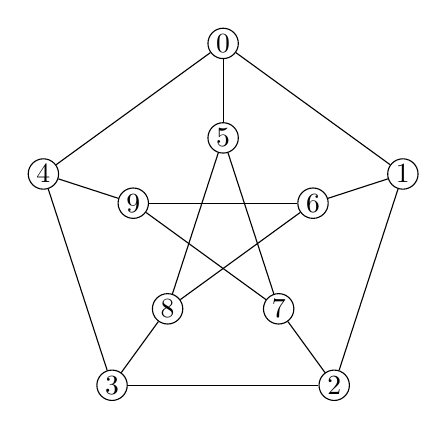
\begin{tikzpicture}[scale=1.2]

% Outer 5-cycle
\foreach \i/\name in {90/0, 18/1, 306/2, 234/3, 162/4}
  \node[draw, circle, inner sep=1pt] (\name) at ({2*cos(\i)}, {2*sin(\i)}) {\name};

% Inner 5-cycle
\foreach \i/\name in {90/5, 18/6, 306/7, 234/8, 162/9}
  \node[draw, circle, inner sep=1pt] (\name) at ({1*cos(\i)}, {1*sin(\i)}) {\name};

% Edges
\foreach \i/\j in {0/1, 1/2, 2/3, 3/4, 4/0} \draw (\i) -- (\j);
\foreach \i/\j in {5/7, 7/9, 9/6, 6/8, 8/5} \draw (\i) -- (\j);
\foreach \i/\j in {0/5, 1/6, 2/7, 3/8, 4/9} \draw (\i) -- (\j);

\end{tikzpicture}
\caption{Petersen graph}
\label{fig:petersen}
\end{minipage}
\hfill
\begin{minipage}{0.45\textwidth}
\centering
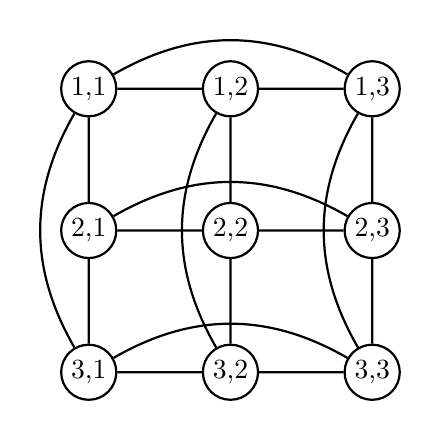
\begin{tikzpicture}[scale=1.2, every node/.style={circle, draw, inner sep=1pt, minimum size=0.7cm}, thick]

% Rook graph R(3)
\node (v11) at (-0.5, 3.5) {1,1}; \node (v12) at (1, 3.5) {1,2}; \node (v13) at (2.5, 3.5) {1,3};
\node (v21) at (-0.5, 2) {2,1}; \node (v22) at (1, 2) {2,2}; \node (v23) at (2.5, 2) {2,3};
\node (v31) at (-0.5, 0.5) {3,1}; \node (v32) at (1, 0.5) {3,2}; \node (v33) at (2.5, 0.5) {3,3};

\foreach \i in {1,2,3} {
  \foreach \j [count=\k from 2] in {1,2} {
    \draw (v\i\j) -- (v\i\k);
  }
}
\foreach \j in {1,2,3} {
  \foreach \i [count=\k from 2] in {1,2} {
    \draw (v\i\j) -- (v\k\j);
  }
}

\draw[bend right] (v11) to (v31);
\draw[bend left] (v11) to (v13);
\draw[bend right] (v13) to (v33);
\draw[bend left] (v31) to (v33);
\draw[bend right] (v12) to (v32);
\draw[bend left] (v21) to (v23);

\end{tikzpicture}
\caption{Rook graph $R(3)$}
\label{fig:rook-graph}
\end{minipage}

\vspace{1.2em}

% Second row: T(4) and T(4) \ {1,2}
\begin{minipage}{0.45\textwidth}
\centering
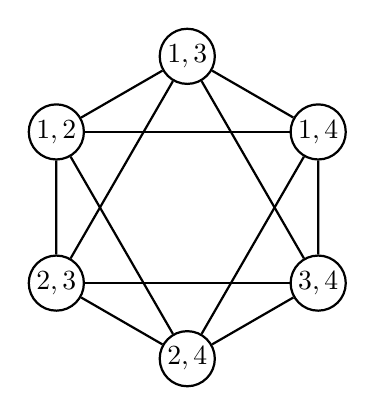
\begin{tikzpicture}[scale=1.2, every node/.style={circle, draw, inner sep=1pt, minimum size=0.7cm}, thick]

\foreach \i/\name in {90/13, 30/14, 330/34, 270/24, 210/23, 150/12}
  \node (l\name) at ({1.6*cos(\i)}, {1.6*sin(\i)}) 
  {$\pgfmathparse{int(\name/10)}\pgfmathresult,\pgfmathparse{int(mod(\name,10))}\pgfmathresult$};

\draw (l12) -- (l13);
\draw (l12) -- (l14);
\draw (l12) -- (l23);
\draw (l12) -- (l24);
\draw (l13) -- (l14);
\draw (l13) -- (l23);
\draw (l13) -- (l34);
\draw (l14) -- (l24);
\draw (l14) -- (l34);
\draw (l23) -- (l24);
\draw (l23) -- (l34);
\draw (l24) -- (l34);

\end{tikzpicture}
\caption{Triangular graph \(T(4)\)}
\label{fig:t4}
\end{minipage}
\hfill
\begin{minipage}{0.45\textwidth}
\centering
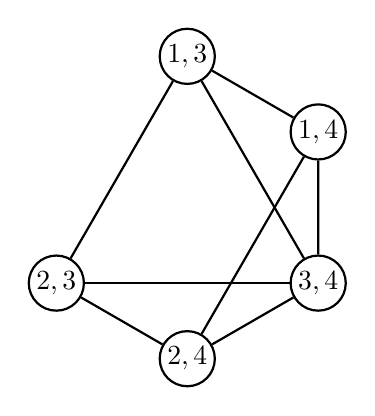
\begin{tikzpicture}[scale=1.2, every node/.style={circle, draw, inner sep=1pt, minimum size=0.7cm}, thick]

\foreach \i/\name in {90/13, 30/14, 330/34, 270/24, 210/23}
  \node (r\name) at ({1.6*cos(\i)}, {1.6*sin(\i)}) 
  {$\pgfmathparse{int(\name/10)}\pgfmathresult,\pgfmathparse{int(mod(\name,10))}\pgfmathresult$};

\draw (r13) -- (r14);
\draw (r13) -- (r23);
\draw (r13) -- (r34);
\draw (r14) -- (r24);
\draw (r14) -- (r34);
\draw (r23) -- (r24);
\draw (r23) -- (r34);
\draw (r24) -- (r34);

\end{tikzpicture}
\caption{$T(4)$ with vertex $\{1,2\}$ deleted}
\label{fig:t4'}
\end{minipage}

% \caption{Top: Petersen and Rook graphs. \quad Bottom: The triangular graph \(T(4)\) and its induced subgraph without vertex \(\{1,2\}\).}
\label{fig:grid-graphs}
\end{figure}












% \begin{figure}[h!]
% \centering
% \begin{tikzpicture}[scale=1.5, every node/.style={circle, draw, inner sep=1.5pt, minimum size=0.8cm}, every path/.style={thick}]

% % Define coordinates for vertices
% \node (v11) at (0, 3) {1,1};
% \node (v12) at (1, 3) {1,2};
% \node (v13) at (2, 3) {1,3};

% \node (v21) at (0, 2) {2,1};
% \node (v22) at (1, 2) {2,2};
% \node (v23) at (2, 2) {2,3};

% \node (v31) at (0, 1) {3,1};
% \node (v32) at (1, 1) {3,2};
% \node (v33) at (2, 1) {3,3};

% % Draw edges for rows
% \foreach \i in {1,2,3} {
%     \foreach \j [count=\k from 2] in {1,2} {
%         \draw (v\i\j) -- (v\i\k);
%     }
% }

% % Draw edges for columns
% \foreach \j in {1,2,3} {
%     \foreach \i [count=\k from 2] in {1,2} {
%         \draw (v\i\j) -- (v\k\j);
%     }
% }

% % Add curved edges to connect the corners
% \draw[bend right] (v11) to (v31); % Connect (1,1) to (3,1)
% \draw[bend left] (v11) to (v13); % Connect (1,1) to (1,3)
% \draw[bend right] (v13) to (v33); % Connect (1,3) to (3,3)
% \draw[bend left] (v31) to (v33); % Connect (3,1) to (3,3)

% \draw[bend right] (v12) to (v32);
% \draw[bend left] (v21) to (v23);

% \end{tikzpicture}
% \caption{The Rook Graph $R(3)$}
% \label{fig:rook-graph}
% \end{figure}

% \begin{figure}[h!]
% \centering

% % --- Petersen Graph ---
% \begin{minipage}{0.45\textwidth}
% \centering
% \begin{tikzpicture}[scale=1]

% % Outer 5-cycle
% \foreach \i/\name in {90/0, 18/1, 306/2, 234/3, 162/4}
%   \node[draw, circle, inner sep=1pt] (\name) at ({2*cos(\i)}, {2*sin(\i)}) {\name};

% % Inner 5-cycle (star points)
% \foreach \i/\name in {90/5, 18/6, 306/7, 234/8, 162/9}
%   \node[draw, circle, inner sep=1pt] (\name) at ({1*cos(\i)}, {1*sin(\i)}) {\name};

% % Outer pentagon edges
% \foreach \i/\j in {0/1, 1/2, 2/3, 3/4, 4/0}
%   \draw (\i) -- (\j);

% % Inner star edges
% \foreach \i/\j in {5/7, 7/9, 9/6, 6/8, 8/5}
%   \draw (\i) -- (\j);

% % Spokes
% \foreach \i/\j in {0/5, 1/6, 2/7, 3/8, 4/9}
%   \draw (\i) -- (\j);

% \end{tikzpicture}
% \caption{Petersen graph}
% \end{minipage}
% \hfill
% % --- Rook Graph ---
% \begin{minipage}{0.45\textwidth}
% \centering
% \begin{tikzpicture}[scale=1.5, every node/.style={circle, draw, inner sep=1.5pt, minimum size=0.8cm}, thick]

% % Nodes
% \node (v11) at (0, 3) {1,1};
% \node (v12) at (1, 3) {1,2};
% \node (v13) at (2, 3) {1,3};

% \node (v21) at (0, 2) {2,1};
% \node (v22) at (1, 2) {2,2};
% \node (v23) at (2, 2) {2,3};

% \node (v31) at (0, 1) {3,1};
% \node (v32) at (1, 1) {3,2};
% \node (v33) at (2, 1) {3,3};

% % Row edges
% \foreach \i in {1,2,3} {
%     \foreach \j [count=\k from 2] in {1,2} {
%         \draw (v\i\j) -- (v\i\k);
%     }
% }

% % Column edges
% \foreach \j in {1,2,3} {
%     \foreach \i [count=\k from 2] in {1,2} {
%         \draw (v\i\j) -- (v\k\j);
%     }
% }

% % Diagonals and curved edges
% \draw[bend right] (v11) to (v31);
% \draw[bend left] (v11) to (v13);
% \draw[bend right] (v13) to (v33);
% \draw[bend left] (v31) to (v33);
% \draw[bend right] (v12) to (v32);
% \draw[bend left] (v21) to (v23);

% \end{tikzpicture}
% \caption{Rook graph $R(3)$}
% \label{fig:rook-graph}
% \end{minipage}

% \label{fig:petersen-vs-rook}
% \end{figure}
% \begin{figure}[h!]
% \centering
% \begin{tikzpicture}[scale=1.2, every node/.style={circle, draw, inner sep=1pt, minimum size=0.7cm}, thick]

% % --- T(4) (on the left) ---
% \foreach \i/\name in {
%   90/13, 30/14, 330/34, 270/24, 210/23, 150/12}
%   \node (l\name) at ({-2.8 + 1.6*cos(\i)}, {1 + 1.6*sin(\i)}) 
%   {$\pgfmathparse{int(mod(\name,10))}\pgfmathresult,\pgfmathparse{int(\name/10)}\pgfmathresult$};

% % Edges of T(4)
% \draw (l12) -- (l13);
% \draw (l12) -- (l14);
% \draw (l12) -- (l23);
% \draw (l12) -- (l24);
% \draw (l13) -- (l14);
% \draw (l13) -- (l23);
% \draw (l13) -- (l34);
% \draw (l14) -- (l24);
% \draw (l14) -- (l34);
% \draw (l23) -- (l24);
% \draw (l23) -- (l34);
% \draw (l24) -- (l34);

% % --- T(4) \ {1,2} (on the right) ---
% \foreach \i/\name in {
%   90/13, 30/14, 330/34, 270/24, 210/23}
%   \node (r\name) at ({2.8 + 1.6*cos(\i)}, {1 + 1.6*sin(\i)}) 
%   {$\pgfmathparse{int(mod(\name,10))}\pgfmathresult,\pgfmathparse{int(\name/10)}\pgfmathresult$};

% % Edges of T(4) \ {1,2}
% \draw (r13) -- (r14);
% \draw (r13) -- (r23);
% \draw (r13) -- (r34);
% \draw (r14) -- (r24);
% \draw (r14) -- (r34);
% \draw (r23) -- (r24);
% \draw (r23) -- (r34);
% \draw (r24) -- (r34);

% \end{tikzpicture}
% \caption{Left: The triangular graph \( T(4) \). \quad Right: The induced subgraph \( T(4) \setminus \{1,2\} \).}
% \label{fig:t4-and-minus12}
% \end{figure}




% \begin{figure}[h!]
% % \centering
% \begin{tikzpicture}[scale=1.6, every node/.style={circle, draw, inner sep=1.5pt, minimum size=0.8cm}, thick]
% % --- K4 (triangle layout, left) ---
% \node (B) at (-3,0) {2};                   % bottom left
% \node (C) at (0,0) {3};                      % bottom right
% \node (D) at (-1.5,2.6) {4};                % top vertex
% \node (A) at (-1.5,1.05) {1};               % center vertex

% % Edges of K4
% \draw (A) -- (B);
% \draw (A) -- (C);
% \draw (A) -- (D);
% \draw (B) -- (C);
% \draw (B) -- (D);
% \draw (C) -- (D);

% % --- T(4) (on the right) ---
% % Place vertices evenly on a circle, shifted right by +4.5 units
% \foreach \i/\name in {
%   90/13, 30/14, 330/34, 270/24, 210/23, 150/12}
%   \node (\name) at ({4.5 + 2*cos(\i)}, {1 + 2*sin(\i)}) 
%   {$\pgfmathparse{int(mod(\name,10))}\pgfmathresult,\pgfmathparse{int(\name/10)}\pgfmathresult$};

% % Draw edges (pairs of 2-subsets that intersect)
% \draw (12) -- (13);
% \draw (12) -- (14);
% \draw (12) -- (23);
% \draw (12) -- (24);
% \draw (13) -- (14);
% \draw (13) -- (23);
% \draw (13) -- (34);
% \draw (14) -- (24);
% \draw (14) -- (34);
% \draw (23) -- (24);
% \draw (23) -- (34);
% \draw (24) -- (34);

% \end{tikzpicture}
% \caption{The complete graph \(K_4\) and its corresponding triangular graph \(T(4)\).}
% \label{fig:k4-and-t4}
% \end{figure}

% \begin{figure}[h]
% \centering
% \begin{tikzpicture}[scale=1]

% % Outer 5-cycle
% \foreach \i/\name in {90/0, 18/1, 306/2, 234/3, 162/4}
%   \node[draw, circle, inner sep=1pt] (\name) at ({2*cos(\i)}, {2*sin(\i)}) {\name};

% % Inner 5-cycle (star points)
% \foreach \i/\name in {90/5, 18/6, 306/7, 234/8, 162/9}
%   \node[draw, circle, inner sep=1pt] (\name) at ({1*cos(\i)}, {1*sin(\i)}) {\name};

% % Outer pentagon edges
% \foreach \i/\j in {0/1, 1/2, 2/3, 3/4, 4/0}
%   \draw (\i) -- (\j);

% % Inner star edges
% \foreach \i/\j in {5/7, 7/9, 9/6, 6/8, 8/5}
%   \draw (\i) -- (\j);

% % Spokes connecting outer and inner nodes
% \foreach \i/\j in {0/5, 1/6, 2/7, 3/8, 4/9}
%   \draw (\i) -- (\j);

% \end{tikzpicture}
% \caption{The Petersen graph.}
% \label{fig:petersen}
% \end{figure}




